\documentclass[oneside,12pt]{book}  % reqno mette i numeri a destra

\usepackage{moresize}  % serve per avere il fonte \HUGE
\usepackage{a4}  % per stampare in formato a4
\usepackage{amssymb,amsfonts,amsmath}  % serve per includere le macro pi`u potenti dell'AMS per le formule 
\usepackage{eucal,mathrsfs} % Per avere un calligrafico piu' bello
\usepackage[british,UKenglish,USenglish,english,american]{babel}  % per  gli a capo secondo le regole dell'italiano
\usepackage{graphicx} % serve per importare le figure in formato jpg, png, pdf
\usepackage{enumerate}  % Utile per creare items personalizzati
\usepackage{color} % Se vuoi usare i colori, altrimenti toglilo
%\usepackage[
%color,
%draft]        % per togliere showkeys sostituire draft con final
%{showkeys}    % molto utile per stampare i nomi che hai dato alle varie label, compaiono nel draft. Nella versione finale 
%                      basta mettere final oppure commentare l'istruzione per togliere le label.
%% 
\usepackage{pdfsync} % molto utile per saltare dal testo al pdf e vicevera.
%%% MIEI
\usepackage{subfigure}
\usepackage{amsmath}
\usepackage{amsthm}
\usepackage[applemac]{inputenc}
\usepackage{listings} 
\usepackage{placeins}


\theoremstyle{plain} 
\newtheorem{thm}{Teorema}[section] 
\newtheorem{cor}[thm]{Corollario} 
\newtheorem{lem}[thm]{Lemma} 
\newtheorem{prop}[thm]{Proposizione} 

\theoremstyle{definition} 
\newtheorem{defn}{Definizione}[chapter] 

\theoremstyle{remark} 
\newtheorem{oss}{Osservazione} 

%%
%%
%%
%%
\newtheorem{teorema}{Teorema}[chapter]  % per cambiare la numerazione
                                        % basta mettere chapter 
\newtheorem{lemma}[teorema]{Lemma}
\newtheorem{corollario}[teorema]{Corollario}
\newtheorem{proposizione}[teorema]{Proposizione}
\newtheorem{osservazione}[teorema]{Osservazione}
\newtheorem{esempio}[teorema]{Esempio}
\newtheorem{definizione}[teorema]{Definizione}
\newtheorem{problema}[teorema]{Problema}
\newtheorem{ipotesi}[teorema]{Ipotesi}
%%
\numberwithin{equation}{chapter} % serve per numerare le formule in accordo ai capitoli.
%%
%% ALTRE MACRO: nel file macro.tex ho messo tutte le macro che sono utili per i vari simboli. Vengono incluse dall'istruzione
%%
\input macro
%%
%% Se non ti servono (ma sono utili) commenta l'input
%%
%%
%%%%%%%%%%%%%%%%%%%%%%%%%%%%%%%%%%%%%%%%%%%%%%%%%%%%%%%%%%%%%%%%%%%%%%%%%%%%
%%
%%                   TITOLO, INDICE
%%
%%%%%%%%%%%%%%%%%%%%%%%%%%%%%%%%%%%%%%%%%%%%%%%%%%%%%%%%%%%%%%%%%%%%%%%%%%%%
%%
%%
\makeindex % serve se vuoi fare un indice delle parole alla fine; altrimenti commenta.
\begin{document}

% Code package
\lstset{language=Matlab} 

\thispagestyle{empty}  % toglie il numero di pagina alla pagina inziale
\begin{center}  % serve per centrare un testo  
  {\Large Politecnico di Milano}\\[12pt]    % serve  per andare a capo lasciando uno spazio voluto.

  {\Huge Progetto di \\
  Numerical Analysis for Partial Differential Equations\\
  e Advanced Programming for Scientific Computing }
\end{center}


\begin{center}    % qui metti il titolo della tesi
  \Huge \bf Virtual Element Method
\end{center}
%
\vspace{12pt}
%
\begin{flushleft}
  \noindent\Large
  Students:\\
  Nicolo\`o Ripamonti \\
  Stefano Savar\`e\\
  
\end{flushleft}
%
% \begin{flushright}
%   \noindent\LARGE
%   Tesi di Laurea di:\\
%   Stefano Savar\`e - Matr.
% \end{flushright}
%
\vspace{364pt}
%
\begin{center}
  \large
  Academic year 2014-2015
\end{center}

\newpage

\tableofcontents  %serve per creare l'indice iniziale

%%
%%
%%%%%%%%%%%%%%%%%%%%%%%%%%%%%%%%%%%%%%%%%%%%%%%%%%%%%%%%%%%%%%%%%%%%%%%%%%%%
%%
%%                   INIZIO DELLA TESI
%%
%%%%%%%%%%%%%%%%%%%%%%%%%%%%%%%%%%%%%%%%%%%%%%%%%%%%%%%%%%%%%%%%%%%%%%%%%%%%

% \part{NOME}    % se devi dividere la tesi in piu parti


\renewcommand{\baselinestretch}{1.5} % se vuoi aumentare l'interlinea; altrimenti commenta.

% istruzioni per le sezioni: \chapter{}, \chapter*{}, \section, \section*
% l'asterisco non mette il numero
%%
 
\addcontentsline{toc}{chapter}{Introduction}  % serve per creare la voce Introduzione nella table of contents iniziale


\chapter{Implementazione}
\label{ch:implementazione}

Descriviamo in questo capitolo il codice da noi sviluppato. Abbiamo
utilizzato il linguaggio C++, secondo la logica della programmazione
ad oggetti. Abbiamo creato un semplice Makefile per automatizzare la
compilazione e abbiamo usato Doxygen per generare automaticamente la
documentazione del codice.
Per la parte di visualizzazione del codice abbiamo invece preferito
creare alcuni script Python, sfruttando la libreria Mayavi per i
grafici 3D.
Abbiamo utilizzato uno stile di codice il possibile coerente per
facilitarne la comprensione.

\section{Panoramica del codice}
\label{sec:panoramica}
Il codice \`e basato su 19 classi e un file main. Sfruttendo le
tecniche del \textit{template programming} dichiarazione e
implementazione delle classi sono entrambe nel file header.
Sono stati usati solamente classi della standard library per rendere
la gestione della memoria pi\`u semplice. In particolare i puntatori,
dove necessari sono stati implementati come shared pointers o weak
pointers. 
Scopo dell'implementazione \`e stato il creare un codice il pi\`u
possibile generale e riutilizzabile. Il codice consente di risolvere
il problema di Laplace con condizioni al bordo di Dirichlet in 2D o 3D
su mesh composte da generici poligoni e poliedri.
Il lavoro \`e diviso idealmente in due parti principali:
\begin{itemize}
\item
\textbf{La mesh:} 7 classi con cui viene modellizzata una qualunque
Mesh 2D o 3D formata da elementi non convessi in generale. La
possibilit\`a nei VEM di trattare figure qualunque ha
reso questa parte piuttosto articolata e computazionalmente non
trascurabile. Il calcolo di specifiche propriet\`a dei
poligoni/poliedri (es. volume, normale esterna) \`e significativamente
pi\`u complesso che nel caso standard, ma nondimeno indispensabile per
la risoluzione del problema.

\item
\textbf{La risoluzione del problema con i VEM:} in questa parte si \`e
cercato dapprima di creare un codice che consenta di risolvere il
problema di Laplace su una mesh qualsiasi a prescindere dal tipo di
solver e dalle condizioni al bordo. Dopo di ch\'e si \`e implementato
il solver per il Virtual Element Method e le condizioni al bordo di
Dirichlet, le uniche trattate in questo progetto.
L'idea di base dell'implementazione di questa parte \`e stata di
creare un codice sufficientemente generale da consentire di modificare
il metodo utilizzato (ad esempio FEM al posto che VEM) semplicemente
scrivendo la parte relativa al solver e non quella relativa al
problema o alle condizioni al bordo.

\end{itemize}


\section{La Mesh}
\label{sec:mesh}
Abbiamo scelto di scrivere da zero il codice per la Mesh per via delle
particolarit\`a dei VEM che richiedono elementi pi\`u generali che nel
classico caso degli Elementi Finiti. Tratto comune a tutte le classi
\`e la presenza di due parametri template, \textit{embedded} e
\textit{real}, che garantiscono flessibilit\`a dal punto di vista
dello spazio scelto (2D o 3D) e della precisione dei numeri a virgola
mobile (double o long double). 

La Mesh in 3 dimensioni \`e stata pensata come un insieme di
poliedri. Ciascuno di questi \`e a sua volta composto da un insieme di
poligoni che a loro volta sono definiti come insieme \textit{ordinato}
di punti. Per facilitare diverse operazioni ciascun poliedro contiene
un vettore di puntatori ai vertici e alle facce e viceversa. Questo
comporta alcune difficolt\`a nel constructor, che sono state superate
con la tecnica dei variadic template e un metodo dedicato
esplicitamente alla creazione di un'istanza. Per i puntatori come
gi\`a detto abbiamo usato gli \textit{shared\_pointer} per facilitare
la gestione della memoria. Non abbiamo usato \textit{unique\_pointers}
in quanto all'interno del programma lo stesso puntatore \`e condiviso
da pi\`u classi.

\subsection{Point e MeshPoint}
Queste 2 classi rappresentano un punto in uno spazio di una
specificata dimensione. La differenza tra le due \`e che la prima \`e
intesa per un punto generico, la seconda per un punto appartenente ad
una mesh. Quest'ultima memorizza al suo interno anche i poligoni e i
poliedri che hanno tale punto come vertice e non \`e stato fornito un
copy constructor. Ha inoltre la possibilit\`a di tener traccia dell'ID
del punto e se tale punto \`e sulla frontiera.

La classe Point viene utilizzata anche per rappresentare un vettore,
sono quindi stati forniti i metodi opportuni, come il calcolo della
norma e il prodotto vettore.

Riportiamo qui l'interfaccia della classe Point e i metodi principali:

\begin{verbatim}
template <long embedded,typename real=double>
class Point {

protected:
    array<real,embedded> coordinates;

public:
    // CONSTRUCTORS
    Point(const array<real,embedded>& inputArray);
    Point(const Point<embedded,real>& inputPoint);
    Point(const MeshPoint<embedded,real>& inputPoint);

    // Constructor with variadic template
    template <typename... Args>
    Point(Args... arguments);

    // STANDARD METHOS
    long maxIndex() const;	//!< Maximum index of the point
    long maxAbsIndex() const;	//!< Maximum index of the point with absolute value
    real norm() const;  //!< L2 norm of the vector
    real normL1() const; //!< L1 norm of the vector

    real& operator[](long index);	//!< Get an element by
reference

    template <long embedded2,typename real2>
    friend Point<embedded2,real2> cross(const Point<embedded2,real2>&
point1, const Point<embedded2,real2>& point2);
\end{verbatim}

\noindent\rule{14cm}{1pt}

Riportiamo l'interfaccia della classe MeshPoint e i metodi principali:

\begin{verbatim}
template <long embedded,typename real=double>
class MeshPoint: public Point<embedded,real> {
protected:
    // PROPERTIES
    long pointID;	//!< ID of the MeshPoint
    real value;		//!< Value in the point after the resolution of the problem
    bool isBoundary;	//<! Tells if the MeshPoint is on the boundary

    vector<weak_ptr<Polygon<embedded, real>>> polygonVector;
    vector<weak_ptr<Polyhedron<embedded,real>>> polyhedronVector;

    // CONSTRUCTORS
    // Constructor with variadic template
    template <typename... Args>
    MeshPoint(Args... arguments);

    // STANDARD METHODS
    void addPolygon(weak_ptr<Polygon<embedded,real>> inputPolygon); 
//!< It insert in polygon vector a new Polygon
    void addPolyhedron(weak_ptr<Polyhedron<embedded,real>> inputPolyhedron);	
//!< It insert in polyhedron vector a new Polyhedron


\end{verbatim}

\subsection{Polygon e Polyhedron}
Queste due classi rappresentano un poligono o un poliedro generico,
non convesso in generale. Entrambi sono da intendersi come componenti
di una mesh, non sono state realizzate due versioni come per point in
quanto non necessarie. Per entrambe l'unico modo per creare una nuova
classe \`e sfruttando il metodo \textit{make\_shared\_Polygon}o
\textit{make\_shared\_Polyhedron}, che restituisce uno shared pointer
all'oggetto e si occupa anche di gestire le connessioni tra questi
oggetti.

Polygon \`e da intendersi come un vettore \textit{ordinato} di Point,
pu\`o essere sia in 2D che in 3D. L'ordine dei punti \`e necessario
sia per il fatto che non \`e possibile individuare un poligono non
convesso da un insieme non ordinato di punti, sia per determinare il
verso della normale. In fase di inizializzazione vengono calcolate le
seguenti quantit\`a, necessarie per il problema numerico:
\begin{itemize}
\item area
\item normale
\item baricentro
\end{itemize}

 Polyhedron invece \`e un vettore \textit{non ordinato} di Polygon. 
In fase di inizializzazione vengono calcolate le seguenti quantit\`a, 
necessarie per il problema numerico:
\begin{itemize}
\item volume 
\item normale esterna
\item baricentro
\end{itemize}
Fa inoltre in modo che le normali delle facce siano orientate
coerentemente.

Riportiamo l'interfaccia della classe Polygon e i metodi principali:

\begin{verbatim}
template <long embedded, typename real=double>
class Polygon: public std::enable_shared_from_this<Polygon<embedded,real>> {
protected:
    // PROPERTIES
    // Vector of ordered vertexes
    vector<shared_ptr<MeshPoint<embedded,real>>> pointVector;
	
    bool isBoundary;	// Tells if the Polygon is on the boundary
    real area;	// \return the area of the Polygon
    Vector<3, real> normal;	// oriented normal to the Polygon
    Point<embedded, real> centroid;	// centroid of the Polygon
    vector<weak_ptr<Polyhedron<embedded,real>>> polyhedronVector;

public:
    // CONSTRUCTORS
    Polygon(const privateStruct &,
const vector<shared_ptr<MeshPoint<embedded,real>>>& vertexVector);
    // Constructor with variadic template.
    template <typename... Args>
    Polygon(const privateStruct&,Args... arguments);

    template <typename... Args>
    static shared_ptr<Polygon<embedded,real>> make_shared_Polygon(Args... arguments);

public:
    // STANDARD METHODS
    // Add a new vertex to the Polygon
    void addPoint(const shared_ptr<MeshPoint<embedded,real>>& p1); 
    // Add a new Polyhedron having this as face
    void addPolyhedron(weak_ptr<Polyhedron<embedded,real>> polyhedron);	
			
    Vector<embedded,real> computeCentroid();
    real computeArea();
    real getDiameter();
    real hTriangle(); // Compute the maximum distance between 2 vertexes.

    shared_ptr<MeshPoint<embedded,real>> isPointAVertex(Point<embedded,real>& point);	
    bool isPointInside(Point<embedded,real>& point);
    array<shared_ptr<MeshPoint<embedded,real>>,2> 
isPointOnBoundary(Point<embedded,real>& point);

    Vector<3,real> computeNormal();
    void switchPointsOrder(); // Invert the orientation of the Polygon

\end{verbatim}

\noindent\rule{14cm}{1pt}

Riportiamo l'interfaccia della classe Polyhedron e i metodi principali:

\begin{verbatim}
template <long embedded, typename real=double>
class Polyhedron: public enable_shared_from_this<Polyhedron<embedded,real>> {

protected:
    // PROPERTIES
    // Stores the faces of the Polyhedron
    vector<shared_ptr<Polygon<embedded,real>>> polygonVector; 
	
    bool isBoundary;	// Tells if the Polygon is on the boundary
    real volume;	// volume of the Polyhedron
    Point<embedded,real> centroid;	// Not the real centroid, 
only the mean of the vertexes.

    // Stores the vertexes of the Polyhedron
    vector<shared_ptr<MeshPoint<embedded,real>>> pointVector;	

public:
    // CONSTRUCTORS
    Polyhedron(const privateStruct&,
const vector<shared_ptr<Polygon<embedded,real>>>& inputPolygonVector);
    // Constructor with variadic template. DO NOT USE.
    template <typename... Args>
    Polyhedron(const privateStruct&,Args... arguments)

    template <typename ...Args>
    static shared_ptr<Polyhedron<embedded, real>>
make_shared_Polyhedron;

    // STANDARD METHODS
    // Add a new vertex to the Polygon
    void addPolygon(shared_ptr<Polygon<embedded,real>>& inputPolygon);
    // Add a new Polyhedron having this as face
    void addPoint(shared_ptr<MeshPoint<embedded,real>>& inputPoint);
    Point<embedded,real> computeCentroid();	// return the centroid
    real computeVolume();	// return the volume of the Polyhedron
    real getDiameter();		// return the maximum distance between 2 Points
    // Makes the normal to each face pointing towards the external of the Polyhedron
    void fixExternalNormal();	
    // Makes the normal of each face pointing in the same direction (or inward or outward)
    void fixFacesOrientation();	
    // Maximum distance between vertexes. Necessary for the mesh.
    real hTriangle();	
    void linkPoints();	// Makes all vertexes pointing to this
    void linkPolygons();  // Makes all Polygons pointing to this

    void switchFacesOrientation();	// Invert the orientation of all faces
    // If a new face is added, also his vertexes are added to the pointVector
    void updatePointVector();	


\end{verbatim}

\subsection{Mesh, Mesh2D e Mesh3D}
Mesh \`e una classe astratta che ha lo scopo di rappresentare
una mesh molto generica (anche ad esempio una superficie in uno spazio
3D). L'idea alla base \`e di memorizzare due vettori, uno di Point e
uno di Polygon o Polyhedron a seconda dello spazio scelto, e di creare
dei metodi base per la lettura di diverse tipologie di file, che poi
verranno implementati opportunamente nelle classi derivate. Sono
presenti anche 2 appositi metodi per tener traccia degli elementi alla
frontiera e per settare eventualmente altre propriet\`a della mesh. Non \`e
stato implementato un costruttore, ma viene fornito un metodo
\textit{initialize} che pu\`o essere chiamato dal costruttore di una
classe derivata per l'inizializzazione.

Mesh2D \`e la classe derivata di Mesh per gestire mesh in 2
dimensioni. Per il rilevamento degli elementi di frontiera si sono
cercati i lati presenti in un solo poligono nella mesh, attraverso
l'introduzione di un \textit{pairVector.}

Mesh3D \`e l'analogo nel caso tridimensionale. Per la maggiore
complessit\`a della mesh abbiamo ritenuto opportuno salvare in un
vettore i puntatori alle facce dei poliedri. Questo ci ha permesso di
ottenere gli elementi di frontiera con un algoritmo simile a quello
del caso 2D, ma confrontando le facce al posto dei lati. In questo
caso l'algoritmo non viene chiamato in \textit{setBoundaryElement}
come in precedenza, ma direttamente all'inizializzazione di ogni nuova
faccia in quanto pi\`u veloce.

Riportiamo l'interfaccia della classe Mesh e i metodi principali:

\begin{verbatim}

template <long embedded,typename baseElement,OpenEnum isOpen=OPEN,
typename real=double>
class Mesh {
protected:
    
    // Vector of Polygon or Polyhedr
    vector<shared_ptr<baseElement>> elementVector;	
    // Vector of the vertexes of each element
    vector<shared_ptr<MeshPoint<embedded,real>>> pointVector;	
	
public:
    long numberOfElements;
    long numberOfPoints;

    virtual real hTriangle();	// paramether h of the Mesh
	
    // Method that calls the functions that read the file
    void initialize(string pointFile,string connection,MeshType meshType=ANYTHING3D);

    // It obtains the pointVector from file
    virtual void setPointVector(string file);	
    // It obtains the elementVector from connections
    virtual void setElementVector(string connections, MeshType meshType);
    
    // Virtual method to keep into account the boundary elements
    virtual void setBoundaryElements()=0;
    //	Virtual method used to set other things, like pointIDs
    virtual void setRemainingThings()=0;

    // methods to set the elementVector
    virtual void setTetrahedronMesh(string connection); 
    virtual void setTriangleMesh(string connection);	
    virtual void setAnything3DMesh(string connection);
    virtual void setAnything2DMesh(string connection);
    virtual void setFileType1Mesh(string connection);
    virtual void setFileType2Mesh(string connection);

    virtual void sort(); //!< Sort the pointVector based on pointID


\end{verbatim}

\noindent\rule{14cm}{1pt}

Riportiamo l'interfaccia della classe Mesh2D e i metodi principali:

\begin{verbatim}
template <typename real=double>
class Mesh2D: public Mesh<2,Polygon<2,real>,OPEN,real> {
private:
    // This is to obtain internal and external points	
    vector<pair<long,long>> pairVector;

public:
    long numberOfBoundaryPoints;
	
    // Constructor with input file
    Mesh2D(string pointFile,string connectionFile,MeshType meshType=ANYTHING2D);

    template <typename... Args >
    shared_ptr<Polygon<2,real>> newPolygon(Args... arguments);

    // Mesh of ANYTHING2D type
    virtual void setAnything2DMesh(string connection);

    virtual void setBoundaryElements();
    virtual void setRemainingThings();
\end{verbatim}

\noindent\rule{14cm}{1pt}

Riportiamo l'interfaccia della classe Mesh3D e i metodi principali:

\begin{verbatim}
template <typename real=double>
class Mesh3D : public Mesh<3, Polyhedron<3,real>, OPEN, real> {
protected:
    // Vector of all the Polyhedron faces
    vector<shared_ptr<Polygon<3,real>>> polygonVector;  

public:
    long numberOfPolygons;
    long numberOfBoundaryPoints;

    // Constructor with input file
    Mesh3D(string pointFile,string connectionFile,MeshType meshType=ANYTHING3D);
	
    // STANDARD METHODS
    // Method to create a Polygon after having read it.
    template <typename... Args >
    shared_ptr<Polygon<3,real>> newFace(Args... arguments);

    virtual void setBoundaryElements();
    virtual void setRemainingThings();

    // Mesh of TETRAHEDRON type
    virtual void setTetrahedronMesh(string connection);
    // Mesh of ANYTHING3D type
    virtual void setAnything3DMesh(string connection);

\end{verbatim}

\section{Il problema Laplaciano e il Solver VEM}
\label{sec:solver}
Per la parte relativa alla risoluzione del problema numerico abbiamo
cercato di scrivere un codice il pi\`u modulare possibile, scorporando
la parte relativa alla modellizzazione del problema da quella relativa
al tipo di solver utilizzato (VEM nel nostro caso) e da quella
relativa alle condizioni al bordo (Dirichlet nel progetto). \`E stato fatto
largo uso della tecnica del \textit{template programming} per
garantire questa modularit\'a. 
Le classi che modellizzano il problema sono infatti classi template in
cui due dei parametri sono il tipo di Solver e le condizioni al bordo.
Vi \`e poi una classe dedicata al calcolo dell'errore.
Per il trattamento di matrici, vettori e sistemi lineari \`e stata
utilizzata la libreria open-source Eigen.

\subsection{Problem e Laplace}
Queste due classi sono relative alla modellizzazione di un problema
numerico. 

Problem \`e una classe astratta che descrive un problema molto generico, che pu\`o
essere risolto attraverso un sistema lineare composto da una matrice
di stiffness e un termine noto. Scopo di Problem \`e di definire
un'interfaccia comune a tutti i metodi e di implementare i metodi
pi\`u generici. In particolare la creazione della matrice di stiffness
e del termine noto sono delegate alle classi figlie mentre viene
implementato un solutore di default del sistema lineare (BiCGSTAB),
che pu\`o volendo essere sovrascritto. Sono anche implementati i
metodi relativi al calcolo dell'errore e all'output su file, comuni per ogni metodo.

Laplace \`e una classe che eredita da Problem il cui scopo \`e invece
di modellare un problema di Laplace lasciando la libert\`a di
scegliere un solutore e delle condizioni al bordo appropriate.  
Questo viene effettuato attraverso due parametri template
\textit{SolverType} e \textit{BoundaryConditionType}, attraverso cui
all'inizializzazione di un'istanza viene passato il tipo di solver e
di condizioni al bordo da utilizzare.
Sono poi implementati i metodi per l'assemblamento del sistema
lineare: questa classe delega alle classi
dedicate a solver e condizioni al bordo il calcolo della matrice di
rigidezza locale, a partire da questa si occupa invece dell'assemblamento di quella
globale.

\noindent\rule{14cm}{1pt}

Riportiamo l'interfaccia della classe Problem e i metodi principali:

\begin{verbatim}
template <long embedded,typename MeshType,typename real=double>
class Problem {
	
protected:
    const MeshType& mesh;	//!< Mesh on which the problem is based

public:
    SparseMatrix<real> stiffnessMatrix;
    VectorX<real> knownTerm;
    VectorX<real> solution;
	
public:
    // General constructor for the Problem
    Problem(const MeshType& inputMesh)

    // Virtual method to compute the stiffness matrix
    virtual void computeStiffnessMatrix()=0;
    // Virtual method to compute the known term
    virtual void computeKnownTerm()=0;	

    virtual void computeSolution();
    virtual void operator()();  // Method to execute the method. FreeFem style.

    //  It displays the error after the computation
    virtual void displayError(std::function<real(Point<embedded,real>&)>
 realSolutionFunction);
    // full output to file 
    virtual void write(string outputPoints,string outputConnections,
string outputSolution);	
    // Output to file of the solution
    virtual void writeSolution(string outputSolution="solution.sol");


\end{verbatim}

\noindent\rule{14cm}{1pt}

Riportiamo l'interfaccia della classe Laplace e i metodi principali:

\begin{verbatim}
template <long embedded,typename MeshType,typename SolverType,
typename BoundaryConditionType,typename real=double>
class Laplace: public Problem<embedded,MeshType,real> {
private:
    real diffusionCoeff;	
public:
    // Vector used to fast build the stifnessMatrix.
    vector<Triplet<real>> tripletList; 
    BoundaryConditionType boundaryCondition;
    SolverType solver;

    // Standard constructor
    Laplace(const MeshType& inputMesh,std::function<real(const Point<embedded,real>&)> 
inputForceTerm,std::function<real(const Point<embedded,real>&)> 
inputBoundaryFunction,real inputDiffusionCoeff=1)

    // General method. It invokes the methods of the Solver.
    void computeStiffnessMatrix();
    // General method. It invokes the methods of the Solver and BoundaryCondition 
    void computeKnownTerm();

\end{verbatim}

\subsection{Monomials e MonomialsPolygon}
Sono due classi accessorie al solutore VEM. Ne diamo una descrizione
ora per rendere pi\`u chiaro il seguito. Dato un elemento di una mesh
denotiamo come monomio
$m_\alpha$ di grado $|\alpha|$ la seguente quantit\`a: 
$$m_\alpha:=\bigg( \frac{\xx-\xx_k}{h_dk} \bigg) ^\alpha$$
dove $\xx_k$ \`e il baricentro dell'elemento e $h_k$ il suo diametro.
Per il solutore VEM di grado 1 \`e necessario valutare tale funzione
nei vertici dell'elemento e calcolarne il gradiente.

Nella classe Monomial sono fornite queste due opzioni.

La classe MonomialPolygon invece serve per calcolare le stesse
quantit\`a nel caso di un poligono immerso in uno spazio 3D.
La differenza principale \`e che mentre nel caso standard il gradiente
\`e un vettore con componenti tutte identiche, in questo caso il
gradiente deve essere proiettato sul piano del poligono da
considerare.

\noindent\rule{14cm}{1pt}

Riportiamo l'interfaccia della classe Monomials e i metodi principali:

\begin{verbatim}
template <long embedded,typename baseElement,typename real=double>
class Monomials {
public:
    const shared_ptr<baseElement>& element;	//!< Element can be Polygon or Polyhedron
    real diameter;  //!< Diameter of the element
    Point<embedded,real> centroid;  //!< Centroid of the element
    // It's the gradient of the monomial. It's 1/diameter
    real gradient;

    // CONSTRUCTOR
    Monomials(const shared_ptr<baseElement>& figure);

    // Function to evaluate the monomial in a point
    real evaluate (const Point<embedded,real>& p, long i);
}

\end{verbatim}



\noindent\rule{14cm}{1pt}

Riportiamo l'interfaccia della classe MonomialsPolygon e i metodi principali:

\begin{verbatim}
template <typename real>
class MonomialsPolygon: public Monomials<3, Polygon<3,real>,real> {
public:
    // these are virtual indexes used to project the Polygon on an appropriate plane
    long indexX;
    long indexY;
    long indexZ;
    Vector<3,real> gradientX;
    Vector<3,real> gradientY;
	
    MonomialsPolygon(const shared_ptr<Polygon<3,real>>& figure); 

    // Function to evaluate the monomial in a point
    real evaluate (const Point<3,real>& p, long i);

\end{verbatim}

\subsection{Solver, SolverVEM, SolverVEM2D e SolverVEM3D}
Queste classi rappresentano la parte relativa al solutore numerico. 
RIguardo la parte sui VEM non ci soffermiamo troppo sulla descrizione
del metodo numerico, che rimandiamo all'apposito capitolo, diamo una
descrizione invece sull'implementazione scelta.

Solver \`e una classe astratta che rappresenta un generico
solver. \`E presente un unico metodo, \textit{computeLocalK}, che
serve a calcolare la matrice di rigidezza locale. \`E dunque una
classe estendibile a qualsiasi metodo numerico riconducibile al
calcolo di una matrice di rigidezza locale su ogni elemento.

Le altre tre classi sono figlie di Solver e implementano il solutore
VEM. Non \`e stato possibile creare un'unica classe per il caso 2D e
3D. Si \`e scelto dunque di creare una nuova classe astratta,
SolverVEM, in cui sono stati implementati i metodi comuni al caso 2 bi
e tridimensionale, e di rimandare a SolverVEM2D e SolverVEM3D
l'implementazione dei pochi metodi rimanenti. 

Il solutore VEM segue il procedimento indicato nell'articolo
\ref{beirao2014hitchhiker} attraverso il calcolo successivo delle
matrici $G$, $B$, $D$, $\Pi^\Delta_\star$, $\Pi^\Delta$ e infine
calcolando $$ \mathbf{K_E^h= (\Pi^\Delta_\star)^T \tilde{G}
  (\Pi^\Delta_\star)+(I-\Pi^\Delta)^T (I-\Pi^\Delta)} $$ 
Sono state inoltre sfruttate le classi Monomials e MonomialsPolygon
per la valutazione dei monomi caratteristici del metodo VEM. 
Il calcolo di $\BB$ e del termine noto \`e stato delegato alle classi
figlie metre il resto \`e implementato direttamente in SolverVEM. Il
caso 3D ha richiesto una pi\`u complessa valutazione dei termini al
bordo. \`E stato necessario calcolare il polinomio interpolante VEM su
ogni faccia, il che causa un aumento notevole del tempo di calcolo.

\noindent\rule{14cm}{1pt}

Riportiamo l'interfaccia della classe Solver e i metodi principali:

\begin{verbatim}
template <long embedded,typename baseElement,typename MatrixType,typename real>
class Solver {
protected:
    std::function<real(const Point<embedded,real>&)> forceTerm;
	
public:
    Solver(std::function<real(const Point<embedded,real>&)> inputForceTerm);

    // Main virtual method. To be implemented in subclasses
    virtual MatrixType computeLocalK(const shared_ptr<baseElement>& element)=0;
	
};

\end{verbatim}

\noindent\rule{14cm}{1pt}

Riportiamo l'interfaccia della classe SolverVEM e i metodi principali:

\begin{verbatim}
template <long embedded,long elementDimension,typename baseElement,
typename MonomialType,typename real=double>
class SolverVEM: public Solver<embedded,baseElement,
Matrix<real,Dynamic,Dynamic>,real> {
protected:
    virtual Matrix<real,elementDimension+1,elementDimension+1> 
computeG(MonomialType& monomial);
    virtual Matrix<real,elementDimension+1,Dynamic> 
computeB(const shared_ptr<baseElement>& polyhedron,MonomialType& monomial)=0;
    virtual Matrix<real,Dynamic,elementDimension+1> 
computeD(MonomialType& monomial);
	
    virtual Matrix<real,elementDimension+1,Dynamic> computePIStar(
Matrix<real,elementDimension+1,elementDimension+1>&G,
Matrix<real,elementDimension+1,Dynamic>&B);
    virtual Matrix<real,Dynamic,Dynamic> computePI(
Matrix<real,elementDimension+1,Dynamic>&PIStar,
Matrix<real,Dynamic,elementDimension+1>&D);
	
public:
    //Basic constructor. A lot of paramethers are given as template.

    SolverVEM(std::function<real(const Point<embedded,real>&)> inputForceTerm);
	
    // This is to compute the local stiffness matrix
    virtual Matrix<real,Dynamic,Dynamic> computeLocalK(const
shared_ptr<baseElement>& element); 
    //!< Virtual method to compute the known term.
    virtual real computeKnownTerm(const shared_ptr<baseElement>&element, 
const shared_ptr<MeshPoint<embedded,real>>& point)=0; 
};

\end{verbatim}

\noindent\rule{14cm}{1pt}

Riportiamo l'interfaccia della classe SolverVEM2D e i metodi principali:

\begin{verbatim}
template <typename real=double>
class SolverVEM2D: public SolverVEM<2,2,Polygon<2,real>,Monomial2D<real>,real> {
public:
    virtual Matrix<real,3,Dynamic> computeB(const shared_ptr<Polygon<2,real>>&
polygon,Monomial2D<real>& monomial);

public:
     SolverVEM2D(std::function<real(const Point<2,real>&)> inputForceTerm);
    
     virtual real computeKnownTerm(const shared_ptr<Polygon<2,real>>& element,
const shared_ptr<MeshPoint<2,real>>& point);
};
\end{verbatim}

\noindent\rule{14cm}{1pt}

Riportiamo l'interfaccia della classe SolverVEM3D e i metodi principali:

\begin{verbatim}
template <typename real=double>
class SolverVEM3D: public SolverVEM<3,3,Polyhedron<3,real>,Monomial3D<real>,real> {
public:
    virtual Matrix<real,3,3> computeGPolygon(MonomialsPolygon<real>& monomial);
    virtual Matrix<real,4,Dynamic> computeB(const shared_ptr<Polyhedron<3,real>>& 
polyhedron,Monomial3D<real>& monomial);
    virtual Matrix<real,3,Dynamic> computeBPolygon(const shared_ptr<Polygon<3,real>>& 
polyhedron,MonomialsPolygon<real>& monomial);
    virtual Matrix<real,Dynamic,3> computeDPolygon(MonomialsPolygon<real>& monomial);
		
    virtual Matrix<real,3,Dynamic> computePIStarPolygon(Matrix<real,3,3>&G,
Matrix<real,3,Dynamic>&B);
	
public:
    SolverVEM3D(std::function<real(const Point<3,real>&)> inputForceTerm);
 
    virtual real computeKnownTerm(const shared_ptr<Polyhedron<3,real>>& element,
const shared_ptr<MeshPoint<3,real>>& point);	
};

\end{verbatim}

\subsection{BoundaryCondition, Dirichlet e Dirichlet3D}

\subsection{Error}

\section{Visualizzazione}
\label{sec:visualizzazione}



\chapter{The finite volume method}
We present in this chapter a theoretical overview of the finite volume
method, focalising on the Lax Friedrichs method and on the Roe
fluxes. 
\section{The Godunov's method}
While the finite difference methods start from the differential form
of the equation the finite volume methods are in general based on the
integral form.
Given a domain $\Omega=\Omega_x\times \Omega_t$ we consider a spatial
and temporal discretisation $(x_j,t^n)=(jh,kn)$ where $h$ and $k$ are
respectively the spatial and temporal grid size.
We consider a conservation law in the more general form:
\begin{equation}
  \label{eq:conservation_law}
  \frac{\partial u}{\partial t}+\frac{\partial f(u)}{\partial x}=0
\end{equation}
with appropriate initial and boundary conditions.
Let us define a cell as $[x_{j-1/2},x_{j+1/2}]\times [t^n,t^{n+1}]$
with $x_{j+1/2}=x_j+h/2$ marking the cell boundaries. 

To proceed we compute the conservation law in integral form:
\begin{equation}
  \label{eq:conservation_law_integral_form}
  \int_{x_{j-1/2}}^{x_{j+1/2}}[u(x,t^{n+1})-u(x,t^n)]dx=-\int_{t^n}^{t^{n+1}}[f(u(x_{j+1/2},t))=f(u(x_{j-1/2},t))]dt
\end{equation}
The basic idea is to rewrite the second integral as the difference of
2 fluxes: $F^{n}_{j+1/2}$ and $F^{n}_{j-1/2}$. 
To pursue this aim we define the cell average:
\begin{equation}
  \label{eq:cell_average}
  \bar{u}^{n}_{j}=\frac{1}{h}\int_{x_{j-1/2}}^{x_{j+1/2}}u(x,t^{n})dt
\end{equation}
and the flux:
\begin{equation}
  \label{eq:generic_flux}
  F^{n}_{j+1/2}=F(\bar{u}^{n}_{j},\bar{u}^{n}_{j+1})=\frac{1}{k}\int_{t^n}^{t^{n+1}}f(u(x_{j+1/2},t))dt
\end{equation}
Through these definition we recover the \textit{finite volume scheme}:
\begin{equation}
  \label{eq:generic_finite_volume}
  \bar{u}^{n+1}_{j}=\bar{u}^{n}_{j}-\frac{k}{h}[F(\bar{u}^{n}_{j},\bar{u}^{n}_{j+1})-F(\bar{u}^{n}_{j-1},\bar{u}^{n}_{j})]
\end{equation}

The scheme is already on \textit{conservative form} by construction.

However the evaluation of the integral of $f(u(x_{j+1/2},t))$ over
$t^n,t^{n+1}$ is not trivial and many possibilities are present.
One of the main possibilities is to reconstruct the value of
$u^*=u(x_{j+1/2},t^n)$ from the nearest value of $\bar{u}^n$ (e.g a
linear trivial interpolation would be
$u^*=\frac{1}{2}(\bar{u}^n_j+\bar{u}^n_{j+1})$). To keep into account
the evolution of the $u^*$ in time we solve the Riemann problem. In
particular note that the CFL condition is sufficient to ensure that
$\bar{u}^n_{j+1/2}$ remain constant during a time step. The problem is
indeed to find the intermediate state of the Riemann problem  between
the 2 states $u_l$ and $u_r$.

\section{The Roe fluxes}
The exact solution of the Riemann problem can be even straightforward in
scalar and linear problems, but in the non linear case it's a lot more
difficult and computationally expensive. Even in some cases the exact
solution cannot be found.

The Roe fluxes is one of the method to achieve this goal (e.g solving
the Riemann problem for a non linear vectorial problem). 
Given the equation \ref{eq:conservation_law} in vectorial form we seek
an approximate numerical flux by the linearisation:
\begin{equation}
  \label{eq:linearization_roe}
  \ff^*=A^*\uu^*
\end{equation}
Assuming that $A^*$ is diagonalisable and using some general results
for the linear Riemann problems we obtain the following expression for
the flux:
\begin{equation}
  \label{eq:roe_flux}
  \ff^*=\frac{\ff(\uu_l)+\ff(\uu_r)}{2} -\frac{1}{2}|A^*|(\uu_r-\uu_l)
\end{equation}
where $|A^*|=S^{-1}|\Lambda | S$.
This will be the formula for the flux that I will use later.
The Lax-Friedrichs flux is quite similar to this. The main difference
is about the matrix $A^*$ that in the formula is replaced by his
maximum eigenvalue in absolute value.

To conclude for the non linear case the matrix $A^*$ has to satisfy
certain condition:
\begin{itemize}
\item
The matrix $A^*$ satisfies
\begin{equation}
  \label{eq:roe_condition1}
  \ff(\uu_r)-\ff(\uu_l)=A^*(\uu_r-\uu_l)
\end{equation}
\item
For each $u$
\begin{equation}
  \label{eq:roe_condition2}
  \lim_{u_l,u_r \to u}A ^*(\uu_l,\uu_r)=\ff'(\uu)
\end{equation}
\item
For each $u_l$ and $u_r$, $A^*(u_l,u_r)$ is diagonalisable and has
only real eigenvalues.
\end{itemize}

\section{Derivation of $A^*$}

\subsection{$A^*$ computation}

To derive $A^*$ for our problem \ref{eq:shallow_water} we start by
defining $\zz=h^{-1/2}\qq$. We consider $\zz$ in the following
form: $$\zz=\begin{pmatrix} \alpha \\ \beta \end{pmatrix}=h^{-1/2}\qq=\begin{pmatrix} h^{1/2} \\ mh^{-1/2} \end{pmatrix} $$
from which we can derive $h=\alpha^2$ and $m=\alpha\beta$.
\\
\\
Substituting this into the definition of f yields
\begin{equation}
  \label{eq:roe_flux_z}
  \gg(\zz)=\ff(\qq(\zz))=\begin{pmatrix} \alpha\beta \\ \beta^2+\frac{1}{2}g\alpha^4 \end{pmatrix}
\end{equation}
From this the following problem follows
\begin{equation}
  \label{eq:shallow_water_z}
  \begin{pmatrix} \alpha \\ \beta \end{pmatrix}_t+\begin{pmatrix} \alpha\beta \\ \beta^2+\frac{1}{2}g\alpha^4 \end{pmatrix}_x=0
\end{equation}
\\
Now suppose $z$ is given by $$\zz=\zz(\mu)=\zz_l+(\zz_r-\zz_l)\mu$$ with $\mu
\in (0,1)$ and define $$C^*=\int_0^1\gg'(\zz(\mu))d\mu$$
With this definition we can write
\begin{equation}
\begin{split}
  \ff(\qq_r)&-\ff(\qq_l)=\gg(\zz_r)-\gg(\zz_l)=\int_0^1\frac{\partial}{\partial
  \mu}(\gg(\zz(\mu)))d\mu \\
&=\int_0^1\gg'(\zz(\mu))\frac{\partial
  \zz}{\partial \mu}(\mu)d\mu
=\int_0^1\gg'(\zz(\mu))d\mu(\zz_r-\zz_l)=C^*(\zz_r-\zz_l)
\end{split}
\end{equation}
To compute now $C^*$ explicitly we consider the Jacobian of
$\gg(\zz)$: $$\gg'(\zz)=\begin{bmatrix} \beta & \alpha \\ 2g\alpha^3
  & 2\beta \end{bmatrix}$$.
As stated befor $C^*$ is the integral from 0 to 1 of
$\gg'(\\z(\mu))$. We thus have to compute:
\begin{equation}
  \label{eq:alpha_integral}
  \int_0^1\alpha(\mu)d\mu=\int_0^1(\alpha_l+(\alpha_r-\alpha_l)\mu)d\mu=\frac{\alpha_r+\alpha_l}{2}=:\bar{\alpha}
\end{equation}
and similarly
\begin{equation}
  \label{eq:beta_integral}
  \int_0^1\beta(\mu)d\mu=\frac{\beta_r+\beta_l}{2}=:\bar{\beta}
\end{equation}
I now have to compute the same integral for $\alpha^3$
\begin{equation}
  \label{eq:alpha_cubic_integral}
  \int_0^1\alpha(\mu)^3d\mu=\int_0^1(\alpha_l+(\alpha_r-\alpha_l)\mu)^3d\mu=...=
  \frac{1}{4}(\alpha_l^3+\alpha_r^3+\alpha_l\alpha_r^2+\alpha_r\alpha_l^2)
\end{equation}
I have omitted some intermediate passages, but the computation is
straightforward. So mixing all together I have obtained an expression
for $C^*$:
\begin{equation}
  \label{eq:c_matrix}
  C^*=\begin{bmatrix} \bar{\beta} & \bar{\alpha} \\ \frac{g}{2} (\alpha_l^3+\alpha_r^3+\alpha_l\alpha_r^2+\alpha_r\alpha_l^2)
  & 2\bar{\beta} \end{bmatrix}
\end{equation}
\newline
In a similar way we have $$\qq_r-\qq_l=\int_0^1\frac{\partial
  \qq}{\partial \zz}(\zz(\mu))d\mu(\zz_r-\zz_l)$$
from which follows $\qq_r-\qq_l=B^*(\zz_r-\zz_l)$. Given
that $$\frac{\partial \qq}{\partial \zz}=\begin{bmatrix} 2\alpha & 0\\
  \beta & \alpha \end{bmatrix}$$ we get
\begin{equation}
  \label{eq:b_matrix}
  B^*=\begin{bmatrix} 2\bar\alpha & 0\\
  \bar\beta & \bar\alpha \end{bmatrix}
\end{equation}
Now we can compute $$A^*=C^*B^{*-1}$$ Through some computation that I
don't report and using the identities $\alpha=h^{1/2}$ and
$\beta=mh^{-1/2}$ I have obtain the following expression:
\begin{equation}
 \label{eq:a_matrix}
  A^*=\begin{bmatrix} 0 & 1\\
  \frac{g}{2}(h_l+h_r)- \left
    (\frac{\frac{m_l}{\sqrt{h_l}}+\frac{m_r}{\sqrt{h_r}}
    }{\sqrt{h_r}+\sqrt{h_l}} \right )^2& 
  2\frac{\frac{m_l}{\sqrt{h_l}}+\frac{m_r}{\sqrt{h_r}} }{\sqrt{h_r}+\sqrt{h_l}} \end{bmatrix}
\end{equation}

\subsection{$|A^*|$ computation}
To compute the decomposition $S\Lambda S^{-1}$ is convenient to
define $$s=\frac{\frac{m_l}{\sqrt{h_l}}+\frac{m_r}{\sqrt{h_r}}
}{\sqrt{h_r}+\sqrt{h_l}} $$
and $$t=\frac{g}{2}(h_l+h_r)$$
With this notation the computation is simpler and we get 
\begin{equation}
  \label{eq:eigenvalues}
  \lambda_{1,2}=s \pm \sqrt{t}
\end{equation}
and
\begin{equation}
  \label{eq:s_matrix}
  S=\begin{bmatrix} 1 & 1\\
  \lambda_1& \lambda_2\end{bmatrix},\quad S^{-1}=\frac{1}{\lambda_1-\lambda_2}\begin{bmatrix} -\lambda_2 & 1\\
  \lambda_1& -1\end{bmatrix}
\end{equation}
Since the computation of eigenvalues and eigenvectors is exact in the
implementation of the method I will use the following formula for
$|A^*|$ 
\begin{equation}
  \label{eq:s_matrix}
  |A^*|=S \left | \begin{bmatrix} \lambda_1 & 0\\
   0 & \lambda_2\end{bmatrix}\right | S^{-1}
\end{equation}
This will reduce significantly the computational cost of the method:
we don't have t compute each time the eigenvector.
For the LF flux instead, it's not necessary to compute $S$, it's
sufficient to get the maximum eigenvalue in absolute value.

\subsection{Checking of the $A^*$ conditions}
As previously stated there are 3 main conditions on $A^*$ that have to
be fulfilled. We examine each of them.
\begin{enumerate}
\item
By construction, $A^*$
satisfies $$\ff(\qq_r)-\ff(\qq_l)=A^*(\qq_r-\qq_l)$$
\item
If we define a function $$\bar
v=\frac{\frac{m_l}{\sqrt{h_l}}+\frac{m_r}{\sqrt{h_r}}
}{\sqrt{h_r}+\sqrt{h_l}}$$ we note that it is continuous in
$h_r$,$h_l$,$m_r$ and $m_l$. Moreover when $h_r=h_l=h$ and $m_r=m_l=m$,
$\bar v$ satisfies $\bar v=m/h$. Therefore
$$\lim_{\qq_l,\qq_r \to \qq }A^*(\qq_l,\qq_r)=\begin{bmatrix} 0 & 1\\
  gh-\left(\frac{m}{h}\right)^2 & 2\frac{m}{h}\end{bmatrix} $$
\item
I have already computed the spectral decomposition of $A^*$, so $A^*$
is diagonalisable. Note that the eigenvalues are all real. In fact $h$
is positive by physical constraint.
\end{enumerate}


\subsection{CFL condition}
The computation of the CFL is quite an easy task in the scalar case
but it's much more difficult in the non linear vectorial case. In the
more general formula the CFL condition state 
\begin{equation}
  \label{eq:cfl_condition}
  k<\frac{h}{c}
\end{equation}
where $k$,$h$ are the time,spacial steps, and $c$ is an appropriate
quantity that have to be computed. In our case $c$ is the maximum
eigenvalue of $A^*$, taken in absolute value. 
We should so compute an estimate for
\begin{equation}
  \label{eq:eiganvalues_bounded}
  \lambda_{1,2} = \frac{\frac{m_l}{\sqrt{h_l}}+\frac{m_r}{\sqrt{h_r}}
  }{\sqrt{h_r}+\sqrt{h_l}}\pm\sqrt{\frac{g}{2}(h_l+h_r)}
\end{equation}
that is our estimate for $c$. 



\chapter{Implementation of Lax-Friedrichs method}
\label{chap:1}
The implementation of Lax-Friedrichs method is described in the last
chapter. In the last section of this chapter there are the most relevant part of code.

\section{Numerical tests}
\subsection{Case with known exact solution}
\label{subsection:1_b}
We started by considering a problem with this initial condition
\begin{equation}
  \label{eq:initial_solution_1b}
  h(x,0)=h_0(x)=1+0.5\sin(\pi x)\quad \quad m(x,0)=m_0(x)=uh_0(x)
\end{equation}
and with
\begin{equation}
  \label{eq:known_term}
  G(x,t)=\begin{bmatrix} \frac{\pi}{2}(u-1)\cos\pi(x-t))\\
   \frac{\pi}{2}\cos\pi(x-t) \left(-u-u^2+gh_0(x-t)\right)\end{bmatrix}
\end{equation}
where $u=0.25$. 
This problem has an exact solution that is
\begin{equation}
  \label{eq:exact_solution}
  h(x,t)=h_0(x-t) \quad \quad m=uh
\end{equation}
I have used in the computation $k=\Delta x/2$ and $T=2$. For the grid
I tested the code on grids with $\Delta x$ between 0.04 and 0.005.

In image \ref{img:lf_1b_solution} we show a comparison between the
numerical found and the exact solution. 
I computed then the error of the numerical solution using the $L_1$
norm. The plot of the error is in figure \ref{img:lf_1b_error}. The
method has, as expected a first order accuracy.
\begin{figure}[h]
\label{img:lf_1b_solution}
\centering
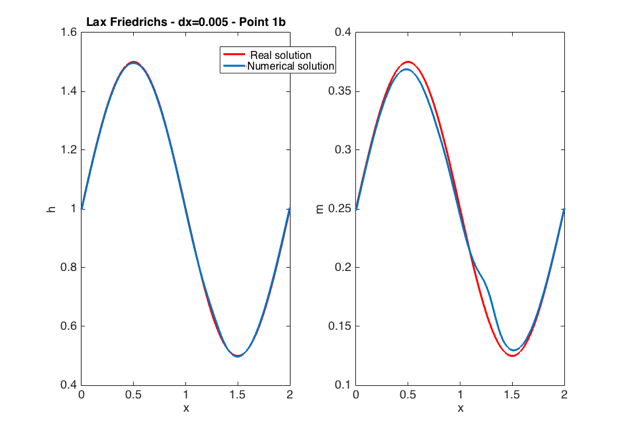
\includegraphics[scale=0.6]{Immagini/LF/1b-solution-2.png}
\caption{Comparison between numerical and exact solution for point
  1b.}
\end{figure}

\begin{figure}[h]
\label{img:lf_1b_error}
\centering
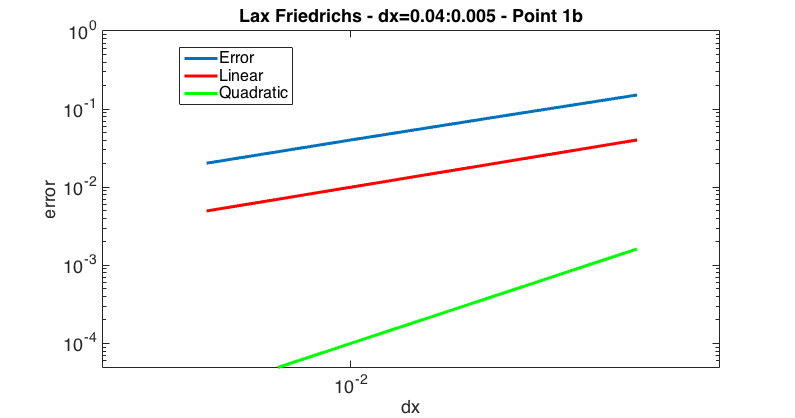
\includegraphics[scale=0.5]{Immagini/LF/1b-error.png}
\caption{Error of the numerical solution with dx varying between 0.04
  and 0.005}
\end{figure}

\subsection{Cases with no exact solution}
\label{subsection:1_c}

Now we run the program with $G=0$ and with these initial functions
\begin{equation}
  \label{eq:initial_solution_1c_1}
  h(x,0)=1-0.1\sin(\pi x)\quad \quad m(x,0)=0
\end{equation}
\begin{equation}
  \label{eq:initial_solution_1c_2}
  h(x,0)=1-0.2\sin(2\pi x)\quad \quad m(x,0)=0.5
\end{equation}
\begin{equation}
  \label{eq:initial_solution_1c_2}
  h(x,0)=\left\{ \begin{matrix} 1.5 & x<1 \\ 0.5 &x>1\end{matrix}\right. \quad \quad m(x,0)=0
\end{equation}
Since we don't have any exact solution for this case we computed the
solution for $\Delta x=0.01/2^3$ and we used it as exact solution. We
then test the order of convergence with $dx=0.08, 0.04, 0.02,
0.01$ for the first case and with $dx=0.04, 0.02,
0.01, 0.005$ for the others to have more evidence on the real order of
convergence. In the following figures we have for each initial
condition the visual comparison with the real solution. Moreover for
each initial condition we show the order of convergence of the scheme
using the $L_1$ norm. We have a first order convergence as expected
for every case.

\begin{figure}[h]
\label{img:lf_1c_1_solution}
\centering
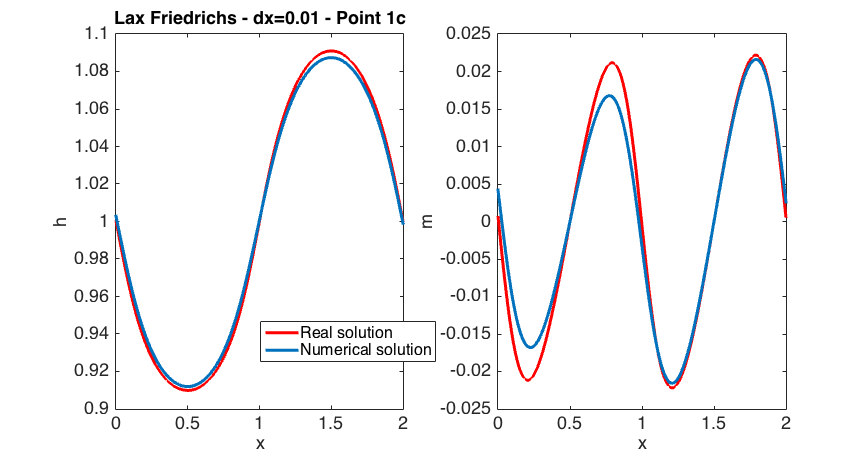
\includegraphics[scale=0.5]{Immagini/LF/1c-1-solution.png}
\caption{Point 1c. Compare exact and numerical solution. Initial condition $h(x,0)=1-0.1\sin(\pi x)$}
\end{figure}

\begin{figure}[h]
\label{img:lf_1c_1_error}
\centering
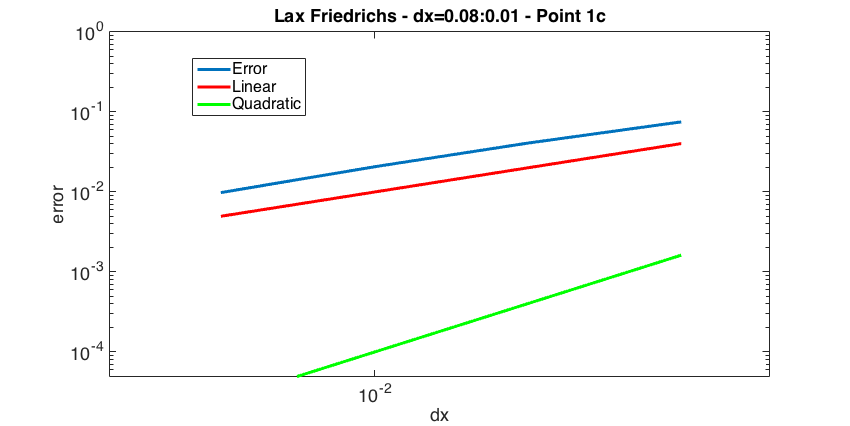
\includegraphics[scale=0.5]{Immagini/LF/1c-1-error.png}
\caption{Point 1c. Error. Initial condition $h(x,0)=1-0.1\sin(\pi x)$}
\end{figure}

\begin{figure}[h]
\label{img:lf_1c_2_solution}
\centering
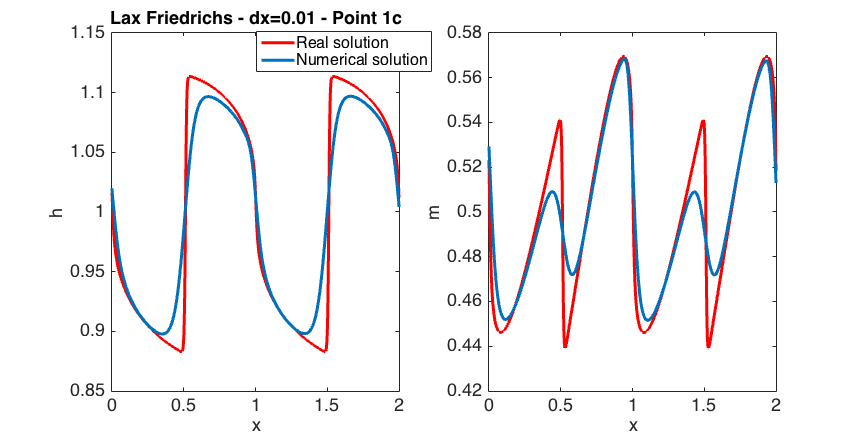
\includegraphics[scale=0.5]{Immagini/LF/1c-2-solution.png}
\caption{Point 1c. Compare exact and numerical solution. Initial condition $h(x,0)=1-0.2\sin(2\pi x)$}
\end{figure}

\begin{figure}[h]
\label{img:lf_1c_2_error}
\centering
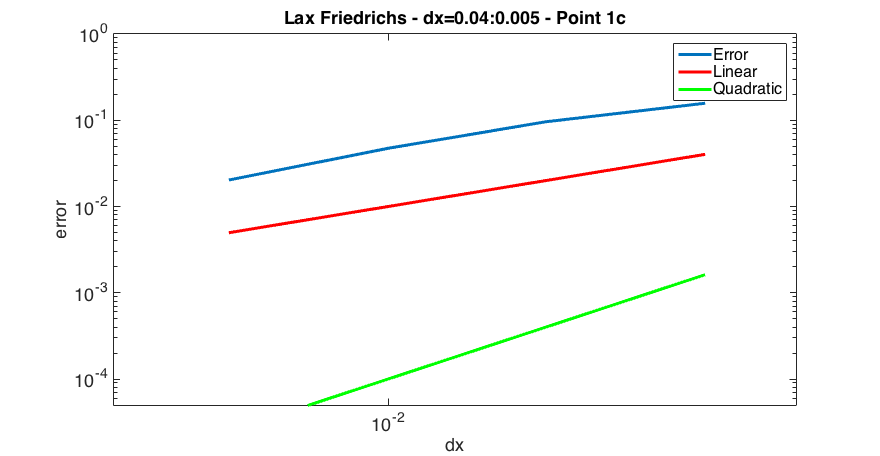
\includegraphics[scale=0.5]{Immagini/LF/1c-2-error.png}
\caption{Point 1c. Error. Initial condition $h(x,0)=1-0.2\sin(2\pi x)$}
\end{figure}

\begin{figure}[h]
\label{img:lf_1c_3_solution}
\centering
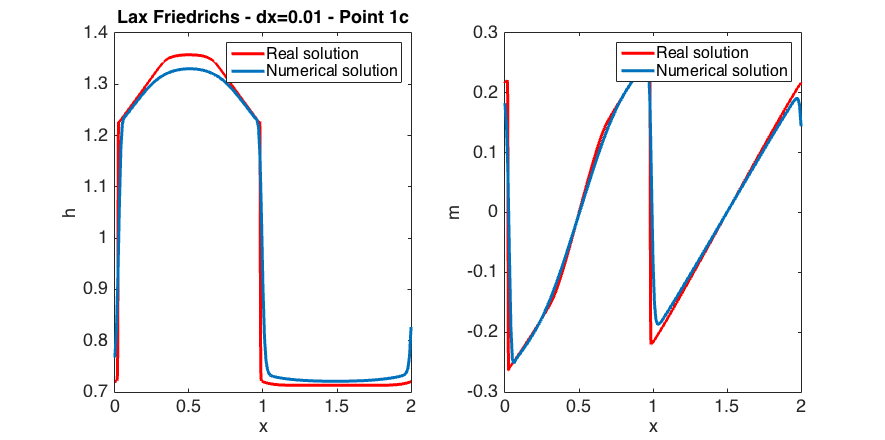
\includegraphics[scale=0.5]{Immagini/LF/1c-3-solution.png}
\caption{Point 1c. Compare exact and numerical solution. Initial
  condition piecewise constant}
\end{figure}

\begin{figure}[h]
\label{img:lf_1c_3_error}
\centering
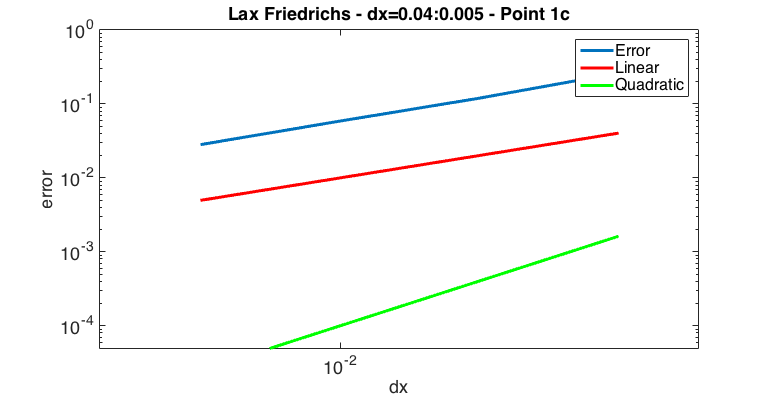
\includegraphics[scale=0.5]{Immagini/LF/1c-3-error.png}
\caption{Point 1c. Error. Initial condition piecewise constant}
\end{figure}

\FloatBarrier
\section{Matlab code}
In this section I provide the Matlab code that I used for the
Lax-Friedrichs solver. I provide the code for the main time loop that
updates the solution at every time step and the code relative to the
computation of the Lax-Friedrichs flux.
\begin{lstlisting}[frame=single]for i=2:length(gridT)
for i=2:length(gridT)
    for j=2:length(gridX)-1
        
        rightFlux=computeLFFlux(h(i-1,j), h(i-1,j+1),
           m(i-1,j), m(i-1,j+1),F);
        leftFlux=computeLFFlux(h(i-1,j-1),h(i-1,j),
           m(i-1,j-1),m(i-1,j),F);

        solution=[h(i-1,j) m(i-1,j)]'
           -dt/dx*(rightFlux-leftFlux)
           +dt*knownTerm(u,gridX(j),gridT(i-1),g);
        h(i,j)=solution(1);
        m(i,j)=solution(2);
        
    end
    
    h(i,1)=h(i,end-1);
    h(i,end)=h(i,2);
    m(i,1)=m(i,end-1);
    m(i,end)=m(i,2);
    
    
end
\end{lstlisting}

\begin{lstlisting}[frame=single]for i=2:length(gridT)
function flux = computeLFFlux( hl,hr,ml,mr,F )

lambda1=( (ml/sqrt(hl)+mr/sqrt(hr))/
   (sqrt(hl)+sqrt(hr))  )^2+sqrt(1/2*(hl+hr));
lambda2=( (ml/sqrt(hl)+mr/sqrt(hr))/
   (sqrt(hl)+sqrt(hr))  )^2 - sqrt(1/2*(hl+hr));

lambda=max(abs([lambda1,lambda2]));

flux=1/2*( F(hl,ml)+F(hr,mr) ) - 1/2*lambda*[hr-hl;mr-ml];


end
\end{lstlisting}

\chapter{Implementation of Godunov's method}
\label{chap:2}

\section{Numerical tests}
In the following subsection we will redo the same numerical
simulations that we did for the Lax-Friedrichs method.
Comparing this method to the Lax-Friedrichs we notice the same order
of convergence, independent from the initial condition. This method
wether the order remains the same provide a better constant. This is
particularly evident comparing the numerical solution with the exact
solution with the same $dx$. 

\subsection{Case with known exact solution}
We reconsider the same initial condition of subsection
\ref{subsection:1_b}. Without repeating all the conditions that are
the same, I show as before the comparison between the numerical and
the exact solution in figure \ref{img:roe_2b_solution} and the
accuracy of the method in figure \ref{img:roe_2b_error}. As expected we have
order 1 again.

\begin{figure}[h]
\label{img:roe_2b_solution}
\centering
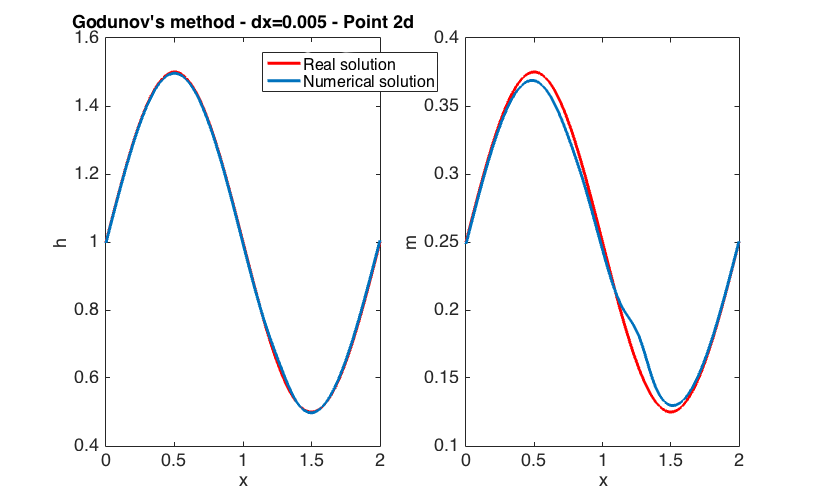
\includegraphics[scale=0.5]{Immagini/LF/2b-solution.png}
\caption{Point 2d. Compare exact and numerical solution. Initial
  condition $h(x,0)=h_0(x)=1+0.5\sin(\pi x)$}
\end{figure}

\begin{figure}[h]
\label{img:roe_2b_error}
\centering
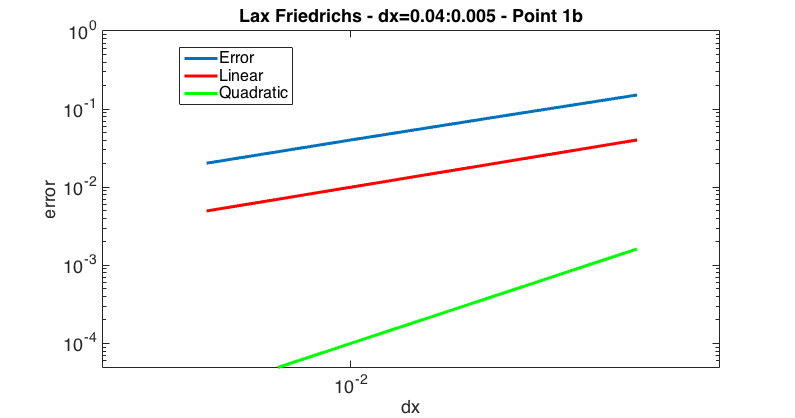
\includegraphics[scale=0.5]{Immagini/LF/1b-error.png}
\caption{Point 2d. Error. Initial condition $h(x,0)=h_0(x)=1+0.5\sin(\pi x)$}
\end{figure}


\subsection{Cases with no exact solution}
We reconsider the same initial condition of subsection
\ref{subsection:1_c}. Since we don't have any exact solution for this case we computed the
solution for $\Delta x=0.01/2^3$ and we used it as exact solution. We
then test the order of convergence with $dx=0.08, 0.04, 0.02,
0.01$ for the first case and with $dx=0.04, 0.02,
0.01, 0.005$ for the others to have more evidence on the real order of
convergence. In the following figures we have for each initial
condition the visual comparison with the real solution. Moreover for
each initial condition we show the order of convergence of the scheme
using the $L_1$ norm. We have a first order convergence as expected
for every case. 


\begin{figure}[h]
\label{img:roe_2c_1_solution}
\centering
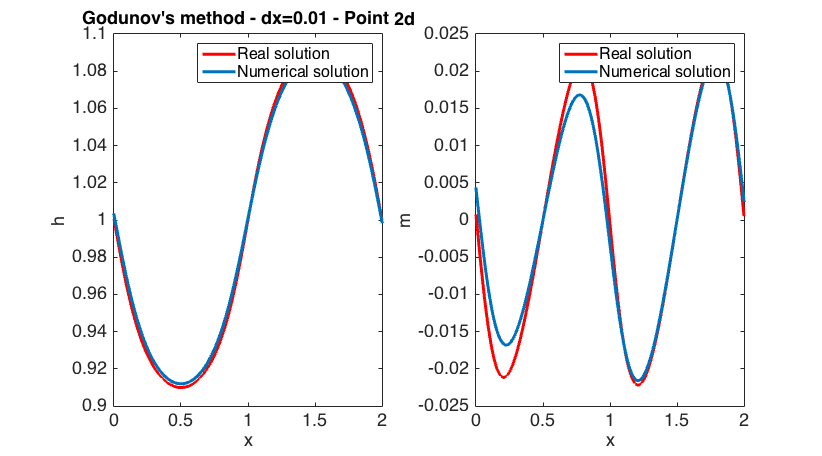
\includegraphics[scale=0.5]{Immagini/LF/2c-1-solution.png}
\caption{Point 2d. Compare exact and numerical solution. Initial condition $h(x,0)=1-0.1\sin(\pi x)$}
\end{figure}

\begin{figure}[h]
\label{img:roe_2c_1_error}
\centering
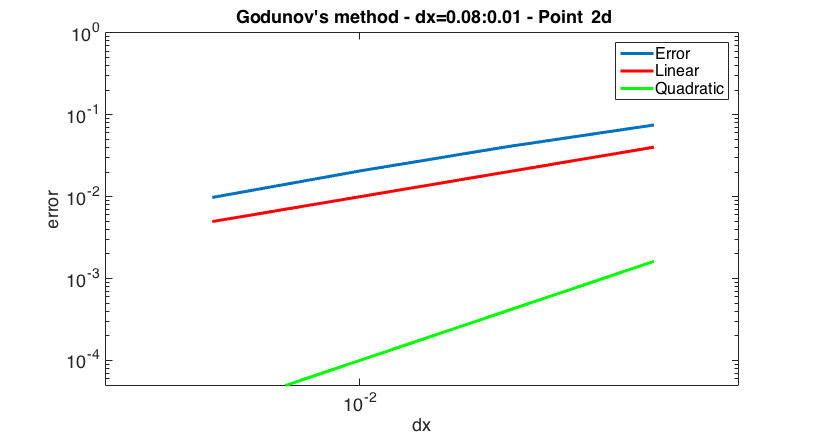
\includegraphics[scale=0.5]{Immagini/LF/2c-1-error.png}
\caption{Point 2d. Error. Initial condition $h(x,0)=1-0.1\sin(\pi x)$}
\end{figure}

\begin{figure}[h]
\label{img:roe_2c_2_solution}
\centering
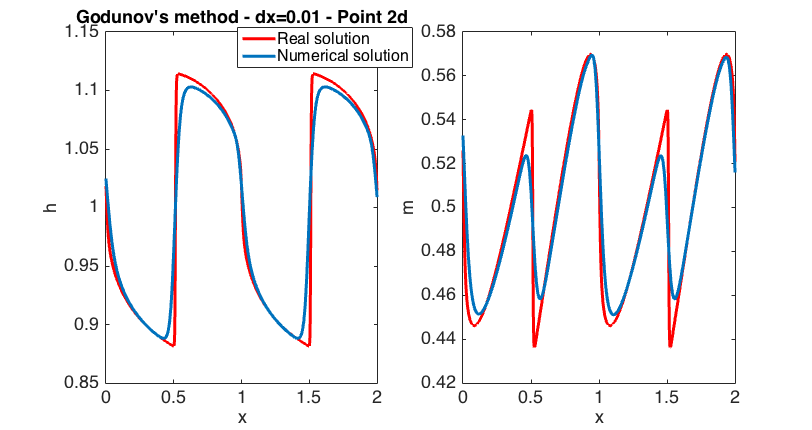
\includegraphics[scale=0.5]{Immagini/LF/2c-2-solution.png}
\caption{Point 2d. Compare exact and numerical solution. Initial condition $h(x,0)=1-0.2\sin(2\pi x)$}
\end{figure}

\begin{figure}[h]
\label{img:roe_2c_2_error}
\centering
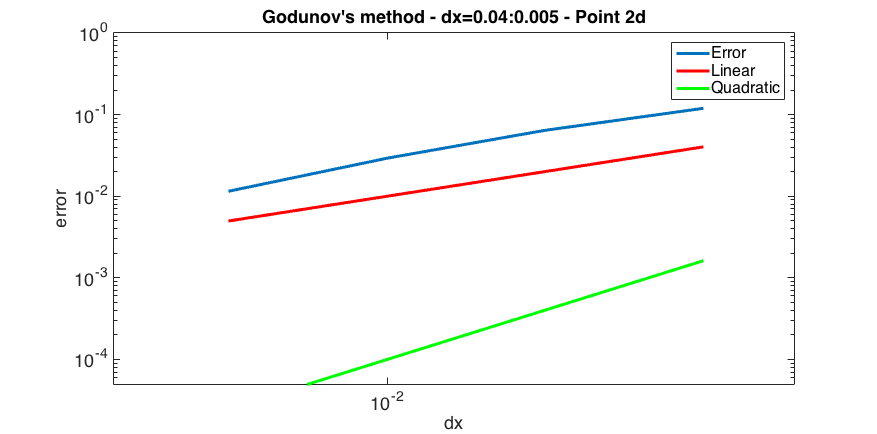
\includegraphics[scale=0.5]{Immagini/LF/2c-2-error.png}
\caption{Point 2d. Error. Initial condition $h(x,0)=1-0.2\sin(2\pi x)$}
\end{figure}

\begin{figure}[h]
\label{img:roe_2c_3_solution}
\centering
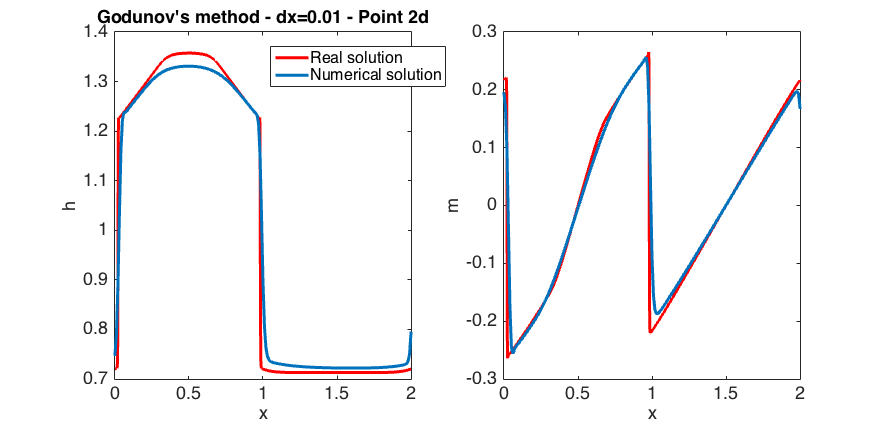
\includegraphics[scale=0.5]{Immagini/LF/2c-3-solution.png}
\caption{Point 2d. Compare exact and numerical solution. Initial
  condition piecewise constant}
\end{figure}

\begin{figure}[h]
\label{img:roe_2c_3_error}
\centering
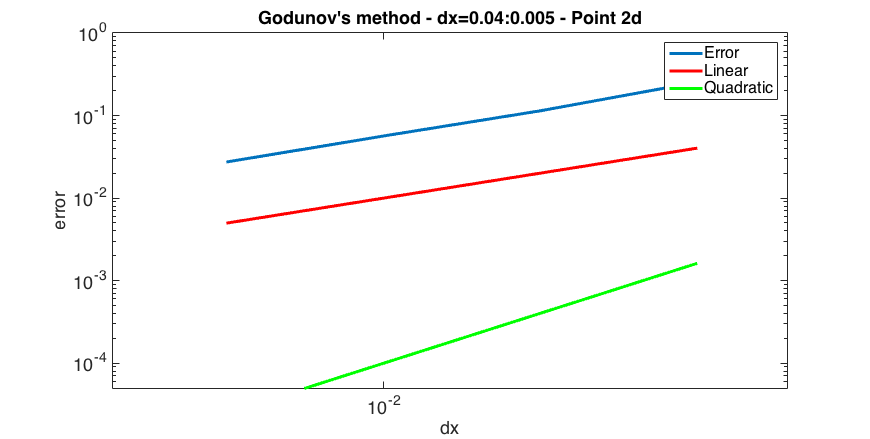
\includegraphics[scale=0.5]{Immagini/LF/2c-3-error.png}
\caption{Point 2d. Error. Initial condition piecewise constant}
\end{figure}

\FloatBarrier
\section{Matlab code}
In this section I provide the Matlab code that I used for the
Godunov's solver. The code for the main time loop that
updates the solution at every time step is the same as the
Lax-Friedrichs one. The following code is the one about the Roe flux.
\begin{lstlisting}[frame=single]for i=2:length(gridT)
function flux = computeROEFlux( hl,hr,ml,mr,F )
lambda1=( (ml/sqrt(hl)+mr/sqrt(hr))/
   (sqrt(hl)+sqrt(hr))  )^2 + sqrt(1/2*(hl+hr));
lambda2=( (ml/sqrt(hl)+mr/sqrt(hr))/
   (sqrt(hl)+sqrt(hr))  )^2 - sqrt(1/2*(hl+hr));

S=[1 1;lambda1 lambda2];
Sinverse=1/(lambda1-lambda2)*[-lambda2 1;lambda1 -1];
EigenMatrix=abs([lambda1 0;0 lambda2]);

A=S*EigenMatrix*Sinverse;

flux=1/2*( F(hl,ml)+F(hr,mr) ) - 1/2*A*[hr-hl;mr-ml];


end
\end{lstlisting}



% \chapter{Un po' di fisiologia}
% \label{chap:3}

% \cite{HodgkinHuxley}
% Nel capitolo \ref{chap:1} abbiamo studiato le basi inutili di matematica. 
% Ora studieremo quelle, ancor meno utili, di fisiologia.

% Prendiamo ad esempio un cuore $\alpha$, una gamba $\beta$, 
% una mano $\mathscr M$, una faccia $\mathcal F$,
% un piede $\mathbb P$, un naso $\mathfrak N$ oppure
% un nasino $\mathsf N$ o un nasone $\nn$.
% Cosa ce ne facciamo? Nulla, appunto.
% Ma grazie alle macro si pu\`o scrivere $\MM$, $\cF$, $\P$, $\frN$, $\sfn$, $\nn$.

% Gli insiemi $\R,\Q,\N,\Z$ sono molto comodi con le macro....


% \medskip
% La bibliografia le vediamo dopo. Comunque si usa il file \emph{bibliografia.bib}
% in cui si mettono tutti i dati bibliografici; ciascuna voce avr\`a una sua label.
% Nel testo quando serve si usa poi il commando \emph{cite}: 
% ad esempio 
% %\cite{Sturm96}
% contiene tutta una matematica che non ti serve...

% Dopo aver compilato il file con \texttt{pdflatex},
% esegui il comando \texttt{bibtex} e poi \texttt{pdflatex} due volte. Alla fine compare la bibliografia aggiornata.

% Trovi il file che uso io, puoi usarlo come esempio per introdurre i testi che ti servono.



% %\appendix  % serve se vuoi creare un appendice 


% %% La bibliografia e' stata compilata e viene richiamata dal file
% %% Paper.bbl; se si vuole ricompilarla con il bibtex occorre
% %% togliere i commenti dalle due linee seguenti
% %% e alla fine aggiungere nel file Paper.bbl la riga
% %%
% %% \addcontentsline{toc}{chapter}{Bibliography}
% %%
% %% subito dopo  \begin{thebibliography}




% \bibliographystyle{siam}
% \addcontentsline{toc}{chapter}{Bibliografia}
% \bibliography{bibliografia}
% %\input{Paper.bbl}


% %% L'indice va stato compilato con l'istruzione
% %% 
% %% makeindex -o tesi.ind tesi.idx
% %%
% %% e viene richimato dal file tesi.ind;
% %% se si vuole ricompilarlo occorre poi 
% %% aggiungere nel file tesi.ind dopo \begin{theindex} la riga
% %% 
% %%   \addcontentsline{toc}{chapter}{Index}
% %%
% %%   
% %\input tesi.in


\end{document}









